\chapter{Introduction}

\section{Portfolio Management}

In financial services, a portfolio is a group of investments including but not limited to stocks, bonds, commodities and real estate. The act of managing said investments is what is called: "Portfolio Management". Formally, this is defined as: "... selecting and overseeing a group of investments that meet the long-term financial objectives and risk tolerance of a client, a company or an institution" \cite{hayes_2022}. Organically, this brings forth the quandary of how does the portfolio manager effectively allocate the assets to best reach its objective? This dissertation will not be focusing specifically on portfolio management theory, it instead will be focused on the concept of volatility in stock returns. To effectively allocate assets, having understanding of volatility is paramount to forecast asset prices. This is defined as: "a statistical measure of the dispersion of returns for a given security or market index ...  [it] is often measured as either the standard deviation or variance between returns from that same security or market index" \cite{hayes_2021}. 

\section{Modelling Asset Returns}
While it is impossible to obtain the true volatility or instantaneous standard deviation of a stock's return tomorrow, models can be created to $\mathbf{simulate}$ the future. Returns can be modelled in two ways: discrete or continuous/logarithmic. Discrete returns are simply $$R_t = \frac{P_t-P_{t-1}}{P_T}$$ or the rate of change between time point $\mathbf{t}$, and time point $\mathbf{t-q}$ where $\mathbf{q}$ is the number of days between price observations.  This research will be considering the daily, continuous/logarithmic returns of stocks on the London Stock Exchange. Formally, a continuous/logarithmic return: $$r_t = ln(\frac{P_t}{P_{t-1}}) = ln(P_t)-ln(P_{t-1})$$ Intuitively, the difference lies in the interval between $\mathbf{t}$ and $\mathbf{t-1}$, where in a discrete return this is simply 1 period, but in a continuous return, this period would be broken in to $\mathbf{k}$ sub intervals, and over those sub intervals the return is continuously compounded, thus yielding.  
$$ 
(1+\frac{rt}{k})^k \Rrightarrow 
||~~ letting~~\mathbf{k}\rightarrow \infty~~ ||~~
~~\lim _{k \to \infty}(1+\frac{rt}{k})^k =e^{rt}
$$ \cite{Popov2022}

\subsection{Time Series}
In statistics, observations that are taken across a set of consecutive time points are considered a "Time Series" \cite{Popov2022}, and therefore when stock market returns are observed, they are classified as a "Financial Time Series". These financial time series observations are considered to have what is called stochastic properties. A stochastic process is a set of observations that follow a random probability distribution and are indexed by time. Formally defined as: $$
X =(X_t)_{t\subset\mathbf{T}}\\
\mu_x(t) = E(X_t) \\ \sigma^2_x(t) = V(X_t) = E(X^2_t)-[\mu_x(t)]^2
$$ The most easily digestible example of a stochastic process is the Gaussian White Noise. This process has a $\mu_x = 0; \sigma^2_x = 1$ and the points are sampled from a normal distribution. $\mathbf{Figure 1.1}$ is a simulated example of the Gaussian White Noise Stochastic process, and shows the points oscillating around the mean of 0 while being randomly distributed generally within 1 standard deviation of the mean. 

\begin{figure}[H]
\centering
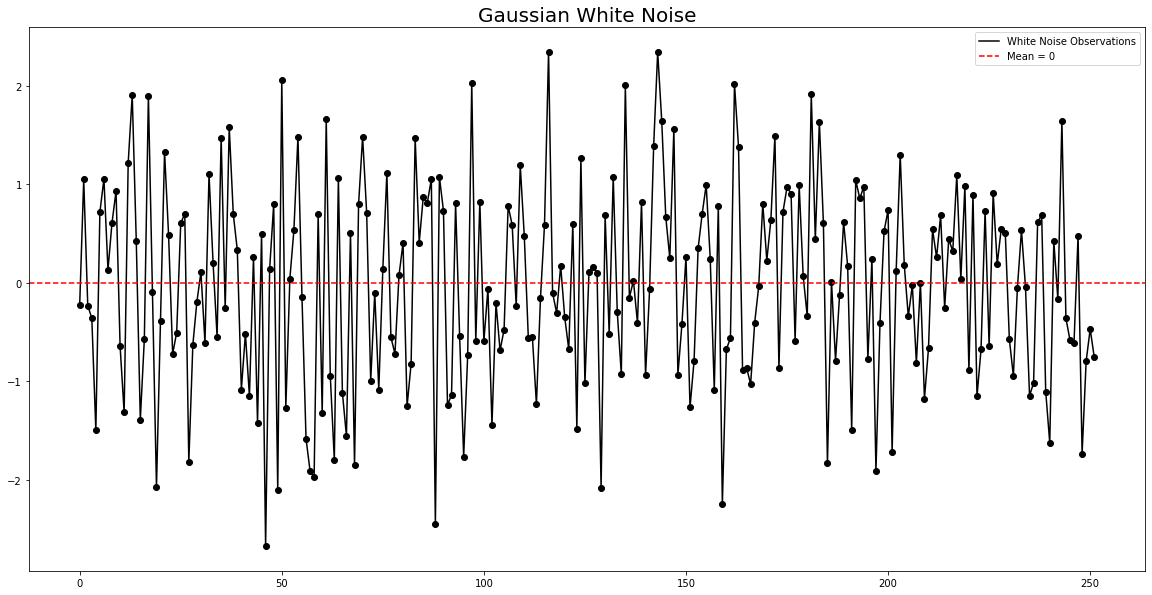
\includegraphics[scale=0.35]{images/GaussianWN.png}
\caption{Random Gaussian White Noise Example}
\label{fig: Gaussian WN}
\end{figure}

\subsection{Properties Financial Data}
Unique to financial data, specifically continuous stock returns, there are properties or "stylized facts" \cite{Popov2022} that are used as a guide.   

\begin{enumerate}
    \item The distribution of the returns are non-normal in two ways:
    \begin{enumerate}
        \item More mass in the tails (fat tails) - greater probability of events further from the mean
        \item There is a higher peak than a normal distribution (leptokurtic) - greater clusters of data at the mean
    \end{enumerate}
    \item Raw returns are uncorrelated, but transforming to squared or absolute, significant autocorrelation is observed
    \item "Volatility Clustering" - if today's return has a large absolute value it tends to be followed by another return with large absolute value, and visa versa with smaller values oof returns.  
\end{enumerate}

\cite{Popov2022}

\section{Motivating Example}
The properties of volatility when modelling returns guide us to the types of models we are using. For example, take Lloyds Banking Group, PLC (LLOY.L)'s returns from 2017 - 2020. Using Maximum Likelihood Estimation, I fit the log returns to a distribution and found they fit best to a Cauchy distribution with a location parameter -0.108 and Scale: 0.76 $\mathbf{Figure 1.2}$. If I assumed mean and volatility to be constant, its expected value is shown by the bottom plot in $\mathbf{Figure 1.3}$. Intuitively this is illogical, financial time series data are dependent on its location in the series, not random observation, this series assumes complete randomness with fat tails that are causing great changes. Comparing the red line in 1.3 to the true Lloyd's returns in the blue line, it is clear the observations volatility's are clustered and the tails are larger than a normal distribution. 
\begin{figure}[H]
\centering
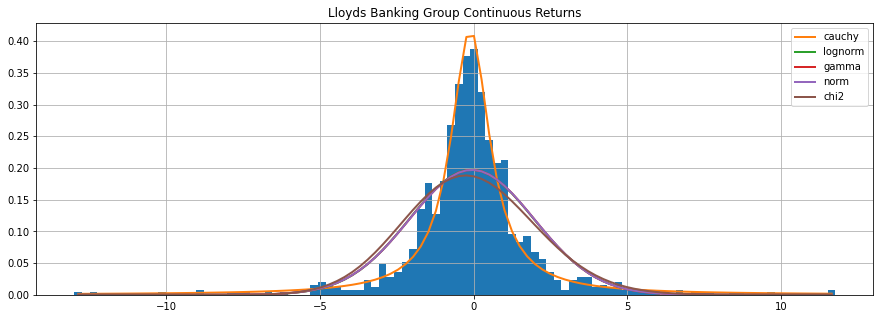
\includegraphics[scale=0.45]{images/LLoyReturnsDistribution.png}
\caption{Lloyds Returns Fitted Distribution}
\label{fig: LLOY Fitted Distribution}
\end{figure}
\begin{figure}[H]
\centering
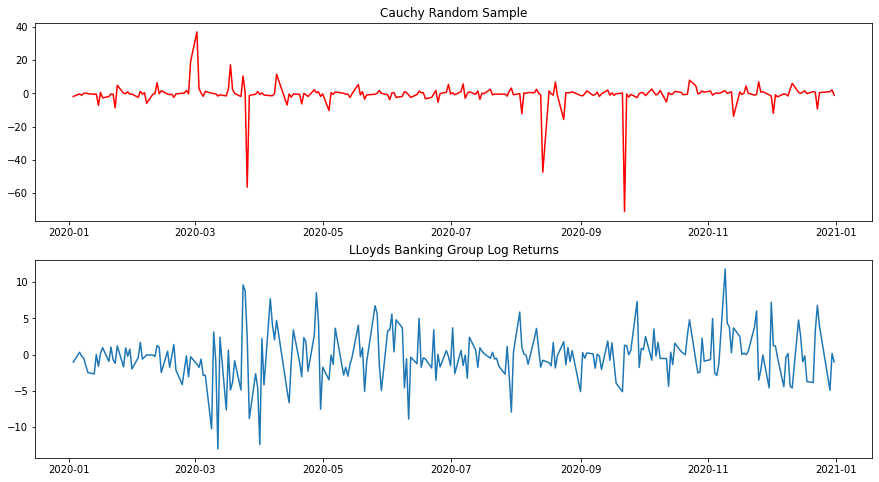
\includegraphics[scale=0.45]{images/LLOYvsCauchy.png}
\caption{Lloyd's Returns vs Cauchy Simulated Returns}
\label{fig: Returns v Cauchy}
\end{figure}
Therefore, this dissertation seeks to find a more accurate and efficient way to model stock market returns to extract the volatility/instantaneous standard deviation.  
\section{Irithmics Exogenous Data}

In an attempt to approach this problem from a novel direction, I will incorporate an exogenous variable into the volatility forecasting model with the hope of increasing the predictive power. Graciously, Irithmics, a U.K. based financial technology and data company donated data it's deep learning machine generated. These data include over a 170 trading days, each with 75-80 a probability density function indexed on each day with the probability value of how likely the deep learning algorithm believes an aggregated group of 250,000 funds will sell/short a specific stock. The corporation's method: 
"Our platform uses state-of-the-art deep learning originally designed to help describe and understand the spread and impact of long-term chronic human diseases, like diabetes. We have applied these technologies to learn from over 250,000 global institutional investors and funds, across hundreds of thousands of portfolios with a combined value of many trillions of dollars" \cite{Irithmics}. The compelling aspect of this exogenous data is it is not objectively correct and therefore the model contains many layers of uncertainty. First, there is the challenge of accurately estimating parameters and hyper parameters, as well as model selection, then whether or not Irithmic's algorithm during the selected time period is an accurate representation of the investors future behavior, and finally if the accurate prediction of the institutions behavior has any significant effect on the volatility of a certain stock's returns. Not only does this problem incorporate the concept of "The Wisdom of Crowds" but also the "Crowd" relationship with stock return volatility.

\section{Data Selection}
\subsection{2020}
There was unprecedented amounts of uncertainty and stock market volatility in 2020 due to the COVID-19 Pandemic. While this was a somber time for humanity, it gives the opportunity to stress test models and model accuracy during extremely uncertain points in time. Generally, forecasting is easy during stable and predictable points in time, but money is made and lost during times where no one knows what to do.  
\subsubsection{FTSE 100}
 Specifically, This analysis will be done on four FTSE 100 Companies from 4 different sectors. The FTSE 100 is the Financial Times Stock Exchange is the largest 100 companies listed in the United Kingdom by market capitalization. I will chose one from: \begin{itemize}
    \item Banking/Finance - LLoyds Banking Group
    \item Technology Vodafone
    \item Automotive - Rolls Royce
    \item Consumer Goods - Tesco
\end{itemize}

\subsection{Forecasting}
Unlike predictions, which rely on a set of non time indexed inputs, forecasting a time series requires always looking forward in time. This poses a larger challenge as fitting, training, and testing models must only focus on predicting out of sample data that lies forward in time. This research will specifically be focused on what is called "nowcasting". The phrase comes from the study of meteorology where weather events are forecast in very near future. The concept will be applied to stock market returns to forecast volatility for what is called a 1 day ahead rolling forecast. 

\section{Wisdom of the Crowds}
\subsection{Book}
In 2004 James Surowiecki, a staff writer at the New Yorker, wrote the book: "The Wisdom of Crowds: Why the Many Are Smarter Than the Few and How Collective Wisdom Shapes Business, Economies, Societies and Nations". The book spoke on his belief that effective and accurate decision making can almost always be improved by aggregating individual forecasts/predictions/decisions rather than individuals making decisions on their own. The simplest example from the book was the old story about Sir Francis Galton, being taken back at a silly carnival game for a crowd to guess the weight of an ox. The mean of the guesses was accurate, while the individual guesses themselves were no good. This is what the wisdom of the crowds or aggregation of the crowd intellegence. This isnt a statistical text, but gives an idea into how the concept of forecast aggregation and crowd wisdom can play into this research paper. The irithmics data aggregates their perceived action from the crowd. On day X, there is a Y\% chance that the 250,000 funds surveyed will short stock Z. If they are shorting stock Z, they are hoping that the stock will go down as they are in the business of making money of their trades. So, the question now becomes, are the crowds wise? are the fund managers aggregated forecasts better than picking say, one fund at Bridgewater Associates, one trader at Jane Street? This paper hopes to incorporate that information, not for stock prices, but to help with the predictions of volatility within the volatilty forecasts.   

The book also acknowledges that all group forecasts aren't created equal. To identify a "wise" crowd there must be: 
\say{\begin{enumerate}
    \item Diversity of Opinion
    \item Independence
    \item Decentralization
    \item Aggregation 
    \item Trust
\end{enumerate}
}\cite{wiki:crowds} 
These ideas for using crowd sourced things can be useful in statistical context, each of these items can be good steps for proper data sampling.   

Conversely, there are some integral failures of the crowd. These intuitively are the inverse of a smart crowd: 
\say{
\begin{enumerate}
    \item Homogeneity
    \item Centralization 
    \item Division
    \item Imitation
    \item Emotionality
\end{enumerate}
} \cite{wiki:crowds} The idea would to be cognizant of the data sampled and the derived forecast one would use. This comes back to the garbage in garbage out modelling, where the data is the most important piece of modelling. One would want to obtain varying forecasts to aggregate from every sense of varying. Socioeconomic Status, , Demographics location time etc etc spatial temporal. 
\subsection{Application}
The compelling aspect is a form of forecast aggregation has already happened and this project seeks extend the aggregation further. The difference is there is also a question of whether or not the forecast itself carries any relevance in the topic. Irithmics aggregated their machine's deep learning prediction on when the aggregation of funds will sell a stock, but is this relevant to the volatility and can this aggregation be aggregated with the empirical forecast. 
